\documentclass[a4paper,11pt]{article}
\usepackage[utf8]{inputenc}
\usepackage{algorithmic}
\usepackage{algorithm}
\usepackage{pst-plot}
\usepackage{graphicx}
\usepackage{endnotes}
\usepackage{graphics}
\usepackage{floatflt}
\usepackage{wrapfig}
\usepackage{amsfonts}
\usepackage{amsmath}
\usepackage{verbatim}
\usepackage{hyperref}
\usepackage{multirow}
\usepackage{pdflscape}

\usepackage{gensymb}

\hypersetup{pdfborder={0 0 0 0}}

\pdfpagewidth 210mm
\pdfpageheight 297mm 
\setlength\topmargin{0mm}
\setlength\headheight{0mm}
\setlength\headsep{0mm}
\setlength\textheight{250mm}	
\setlength\textwidth{159.2mm}
\setlength\oddsidemargin{0mm}
\setlength\evensidemargin{0mm}
\setlength\parindent{7mm}
\setlength\parskip{0mm}

\newenvironment{exercise}[3]{\paragraph{Exercise #1: #2 \textsc{(#3pt)}}\ \\}{
\medskip}
\newcommand{\question}[2]{\setlength\parindent{0mm}\ \\$\mathbf{Q_#1:}$ #2\ \\}

\author{\large{Aqeel Labash, Ardi Tampuu, Dainel Majoral, Ilya Kuzovkin, Raul Vicente}}
\title{\huge{Introduction to Computational Neuroscience}\\\LARGE{Practice II: Data Analysis - Continuous and Spiking data}}

\begin{document}
\maketitle
\ \\
\section{Introduction}
In this practice session we go through how to work with recordings from brain areas (EEG) and individual cells (intracranial recording, spiking data). In the lecture we also covered some other ways of recording brain activity, such as fMRI and MEG. We do not have the time to look at the data from these imaging techniques, but if you find them fascinating, you can work with them in your course project.

\section{EEG data}
Those who made it to the psychology lab visit on Monday, already know how recording EEG (Electroencephalography) signal looks like. For those who were not present: electrodes are placed on different parts of your head and electrical signal is recorded from them. Certain electrodes (on the earlobes, face) do not record the brain activity but are instead used as a reference to filter out noise caused by to muscle activity and electrical signals in the room. When all the electrodes are attached the person looks like this:\\
\begin{center}
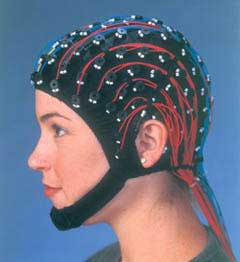
\includegraphics[width=6cm]{eeg.jpg}
\end{center}
After some preprocessing (filtering out noise with the help of reference electrodes), this is how an usual EEG recording of one channel (signal from one electrode is called a channel) looks like:
\begin{figure}[H]
   \centering
   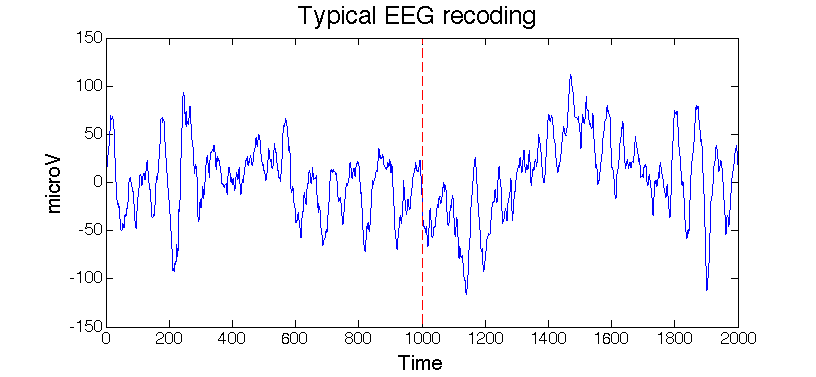
\includegraphics[width=0.8\textwidth]{eegrecording.png} 
  \caption{On the $x$ axis there is time, on the $y$ axis strength of the recorded signal in $\mu$V. The dashed line at the time point $x=1000$ is the moment when the \emph{stimulus} (picture) was shown to the test subject.}
\end{figure}


%
% ERP
%
\begin{exercise}{1}{Event Related Potential (ERP)}{1}
Event related potentials refer to changes in the brain activity in response to certain events. For example, we expect some change in activity of some regions after a person hears a sound.

On the plot above, the test subject was presented with a stimulus at T=1000. Nevertheless, from the plot above one cannot conclude that showing the stimulus had any considerable effect on the subject's brain activity (as measured by this specific electrode). Even though there seems to be a voltage increase starting at T=1200 and ending at the T=1500, it could be a random event not related to the stimulus. Clearly the signal is very noisy.

To remove the noise and reach conclusions on the effect of the stimulus, scientists conduct the same experiment several times and then average the results. In each trial the noise is different and will cancel out if we average over trials. Therefore the brain response, if it is there, will reveal itself much more clearly.

In the \texttt{data} folder you have file \texttt{erptrials.csv}. One row is one trial recorded for 2 seconds with sampling rate of 1000 Hz. The stimulus was shown at the time point 1000 (1 second). There are 79 trials in this file. Your task is to plot an average of all 79 trials to see that there is a clear ERP response or not. Also add a red vertical line at T=1000 like on Figure1. Respond to the following questions: i) How many milliseconds after the stimulus presentation does the ERP happen? ii) How long does it take for the EEG signal to return to normal range?

In your response you are supposed to include the code used for generating the plot and the plot itself, with title and axis names. 
\end{exercise}

%
% Apply fourier
%
\begin{exercise}{2}{Frequency Analysis}{2}
The most popular operation that you can do with continuous brain data such as EEG is converting it from the \emph{time domain} to the \emph{frequency domain}. Due to the fact that any function can be represented as a sum of sinusoids (Fourier transform) we can decompose our signal into such sinusoids and observe from which frequency components it consists. In terms of the brain data such transformation makes particular sense, because of the \emph{brain rhythms} -- different frequencies of the firings of the neurons are related to the different kinds of mental activity\footnote{\url{http://en.wikipedia.org/wiki/Electroencephalography\#Wave_patterns}}.

\ \\
In this exercise we will plot the \emph{power spectrum} (like the two plots below) and see how \emph{alpha wave} (brain oscillation at 8-13Hz) emerges when the test subject's eyes are closed. In the \texttt{data} folder you can find two files: \texttt{eyes\_open.csv} and \texttt{eyes\_closed.csv}. The data is recorded from the channel \texttt{Pz} (you can google where it is located). One row contains 4 seconds of the signal, sampling rate is 512. Each file has 15 recordings.

\ \\
Your task is to perform Fourier analysis on both datasets, plot power spectra and compare the results. Do it as follows:
\begin{enumerate}
	\item Plot some of the signals just to see how they look like.
	\item For each recorded signal (2048 data points):
		\begin{enumerate}
			\item Use \texttt{fft(signal)} to compute power spectrum of this signal. You will get a vector of complex numbers.
			\item Use \texttt{abs(result\_of\_fft)} to obtain the magnitude\footnote{\url{http://www.mathworks.se/help/matlab/ref/abs.html}}. \texttt{abs(result\_of\_fft)}$^2$ will give you \emph{power}.
		\end{enumerate}
	\item Sum together the 15 power spectrum distributions, that you got from the previous step.
	\item And divide the resulting vector by 15 to obtain the average.
	\item Plot it. You will see that the right part of the graph is mirror image of the left part. Discard the right part.
	\item Your $x$ axis goes from 1 to 1024, which does not correspond to actual frequencies. Compute correct $x$ axis as follows:
		\begin{verbatim}
		dt = 1/512;             % time step length in ms
df = 1/4;               % frequency step in Hz, 4 corresponds to 
                        % the length of recording
fNQ = 1/dt/2;           % fNQ is the maximal frequency, in our case it is
                        % 256 if you have discarded part of the data in step 5 
xaxis = (0:df:fNQ-df);  % points for your X axis, should be of the same length 
                        % as the vector of frequencies
		\end{verbatim}
	\item And plot it again
		\begin{verbatim}
		plot(xaxis, powers_average);
		\end{verbatim}
		Now your axis goes from 0 to 256 (or 512 if you did not discard the right side of the graph) with step of 0.25. This corresponds to the frequency range \texttt{pow} function produced.
\end{enumerate}

\ \\
After making the plot more beautiful and focusing only on the range from 0 to 30 Hz you should obtain a result that looks something like this:
\begin{figure}[H]
   \centering
   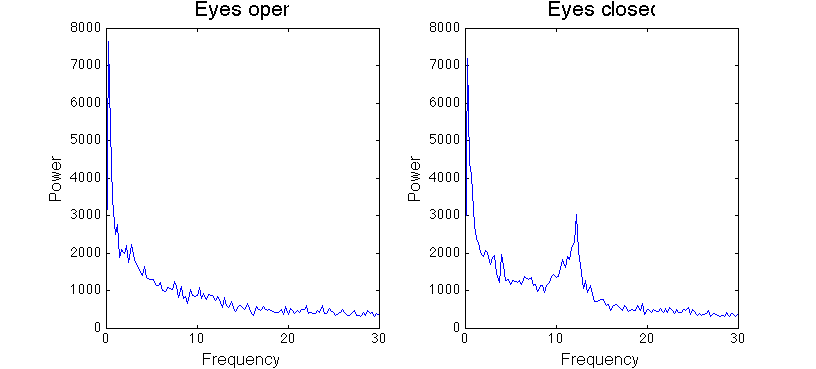
\includegraphics[width=0.7\textwidth]{fouriereyes.png} 
\end{figure}
\end{exercise}

\section{Part II: Spiking Data}
I the first part we looked at continuous brain data: strength of the EEG signal was changing over the time. Another very popular form of data, obtained when we insert electrodes inside the brain and record the activity of individual neurons, is \emph{spiking} data. The concept is very simple: we attach a sensor to the neuron and whenever the neuron emits and action potential (aka "fires") we write a ``1" into our data file, otherwise we write a ``0". The resulting data shows us for each time point (in our case each millisecond) whether the neuron has fired or not.\\
\ \\
\textbf{Dataset}

\begin{wrapfigure}{r}{0.3\textwidth}
	\centering
	\vspace{-12pt}
	
\includegraphics[width=0.15\textwidth]{orientationstimulus.jpg}
	\caption{Example of the stimulus. During the actual experiment the bars are moving.}
	\label{fig:stimulusexample}
	\vspace{-5pt}
\end{wrapfigure}
The dataset we will be working with has the spiking data recorded while the mouse was presented with a stimulus: moving bars on the screen, which can have different orientations. On Figure \ref{fig:stimulusexample} you can see an example: white and black bars are tilted (\emph{orientation}). The bars also move in the direction perpendicular to the tilt during the experiment. The spiking activity is recorded from 72 neurons and we want to find whether different neurons react differently to moving bars with different orientations. Have a look at Figure \ref{fig:orientationresponse} -- spiking pattern of this particular neuron seems to indicate that this neuron is more active when the bar is tilted $45\degree$ clockwise from the horizontal position. And its activity fades when the orientation changes away from 45. We would like to rediscover from the data, that indeed different neurons respond differently to different orientations.
\begin{figure}[H]
	\centering
	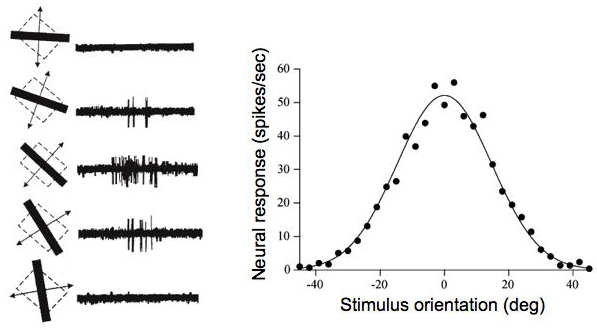
\includegraphics[width=0.7\textwidth]{orientation.jpg} 
	\caption{Neuronal response to different orientations of the bar.}
	\label{fig:orientationresponse}
\end{figure}
\textbf{NB:} Note that in the dataset we have 13 stimuli (13 orientations), but the first one should be ignored (it has orientation $-1\degree$). So you should only use the other 12.



\begin{exercise}{3}{Raster plots}{2}

Let us start by plotting some spiking data. Under the \texttt{data/lgn} folder you have recordings from 72 neurons of a mouse. \texttt{Matlab/Octave} users can use .mat files in the \texttt{matlab} folder, the same data is available in the plain text format in the \texttt{plain} folder.

\texttt{Matlab} files have names \texttt{mlgnori\_NN.mat} where \texttt{NN} is the number of the neuron. When you load it to your environment you will find that each file has a structure with two elements: \texttt{spktimes} and \texttt{stim}. The first one is $M\times N \times T$ matrix where $M$ is the number of different stimuli, $N$ is the number of trials and $T$ is the time in milliseconds. So this is a 3-dimensional matrix containing values 0 (no spike) and 1 (spike) for every millisecond in every trial for every stimulus. A value at position (m,n,t) will therefore tell you if this neuron was active at time t, in trial n of stimulus m. The second element, \texttt{stim}, describes the stimulus. Open it and you will see what information is in there.

If you do not use \texttt{Matlab}, then it is easier for you to use the plain text files. They have names \texttt{neuron\_NN} \texttt{\_stimulus\_SS.csv} where \texttt{NN} is the number of the neuron and \texttt{SS} is the number of the stimulus. Inside each file one line represents one trial. For each millisecond it has value 0 (no spike) or 1 (spike). Files with names \texttt{stimulus\_SS.csv} describe the stimulus: they hold four values:
\begin{enumerate}
\itemsep 0em
	\item Time before the stimulus (in seconds).
	\item Duration of the stimulus (in seconds).
	\item Time after the stimulus (in seconds).
	\item Orientation of the stimulus (in degrees).
\end{enumerate}

\textbf{Hint: } There is some code in the \emph{code} folder .
\textbf{Your task is} to take any of the neurons and plot all trials as a raster plot (see Figure \ref{fig:raster_plot}). You will notice that neuronal response to the stimulus varies a lot (lot of noise!), this is why you usually need several trials.
\begin{figure}[H]
   \centering
   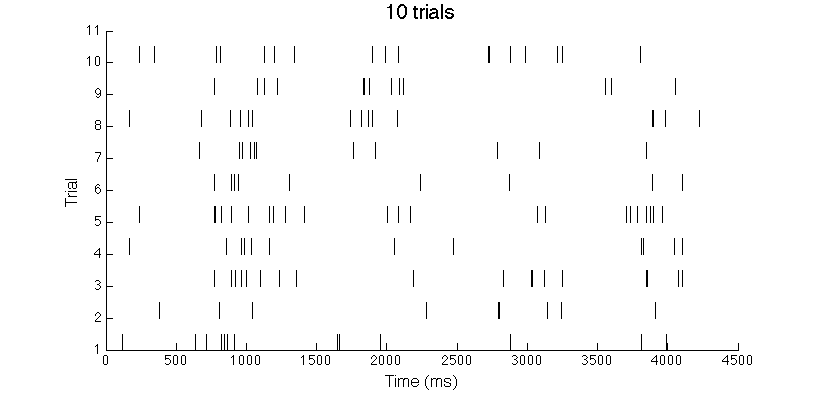
\includegraphics[width=0.7\textwidth]{raster10tr.png} 
   \caption{Raster plot of 10 trials on the same neuron.}
   \label{fig:raster_plot}
\end{figure}
On the $X$ axis we have time and on the $Y$ axis trials. A vertical bar indicates a spike in that trial. To draw a vertical line in \texttt{Matlab} you can use
\begin{verbatim}
	line([t t], [tr tr+0.5], 'Color', 'k');
\end{verbatim}
where \texttt{t} is the time and \texttt{tr} is the number of the trial. If necessary modify the length and width of the bars to make the raster plot more readable.
\ \\

The next step is to \textbf{create two more raster plots}. The first one will illustrate the behaviour of all the neurons under the same stimulus, while the other one will have responses of the same neuron but to the different stimuli.\\

\textbf{Create the following two plots:} 
\begin{enumerate}
	\item Raster plot, where on $X$ axis we have time and on $Y$ axis we have all 72 neurons. Vertical bars are the responses to a stimulus (choose any) by the corresponding neuron in any of the trials (!). Please note that in our dataset different recordings have different length, but this should not be a problem. \textbf{(neuron to neuron variability)}
	\item Raster plot, where on $Y$ axis we have all 12 stimuli and bars are the responses from the same neuron (choose any). \textbf{(variability across stimuli)}
\end{enumerate}

\textbf{Hint: }\emph{For the first of the two plots we need to average spiking data over the trials so that each neuron would be represented by only one vector, not 10. Simplest way to do that is just to add trials together. Let us say that you have 10 trials, and each of them is a vector of 4500 time points. You just sum those vectors together to obtain one vector of length 4500. After that replace all values which are grater than 1 with 1 (meaning if there was a spike in that time point in at least one of the trials)}.

\end{exercise}


\begin{exercise}{4}{Tuning Curve as Rose Diagram}{2}

\textbf{Hint: } There is some code for this exercise in \emph{code} folder.

From the lecture you must be familiar with the term \emph{receptive field}. \emph{Tuning curve} is a plot that helps to describe the receptive field of a neuron with respect to some variable - how strongly does the neuron respond (how often it fires) if we give the variable different values. Figure 3 describes how a neuron's response varies for different orientations of the bar, the plot on the right is the tuning curve of this neuron (with respect to orientation).

For orientations of bars there is a really neat way to visualize the tuning curve. This visualization method is called \emph{rose chart} or \emph{angle histogram}. You can see an example on Figure \ref{fig:rosediag}. The idea is that the values are placed on the circumference on the circle and the length of the sector is determined by the number of times the value appears in the list. It is like a histogram drawn in circle.

In our case it allows to represent our data in a much more natural way because different orientations form a circle. In our case the lengths of the sectors correspond to sum of spikes in this orientation. There are rose charts for some of the neurons on Figure \ref{fig:rosediag}. We can clearly see that neuron 8 reacts more to the orientation of $0\degree$, the neuron 6 is most active in the range of $270\degree$ to $330\degree$ and so on.

\begin{figure}[H]
   \centering
   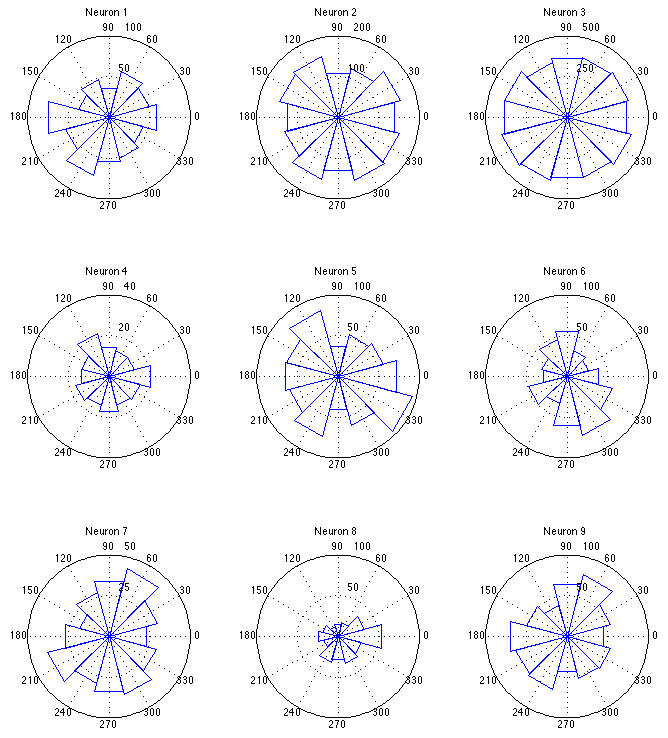
\includegraphics[width=0.65\textwidth]{rosediag.png} 
   \caption{Rose diagram: the number of spikes for each of the 12 orientations.}
   \label{fig:rosediag}
\end{figure}

\textbf{Your task is} to produce similar plot for any 9 neurons (not the same ones as on previous figure). To produce a plot for one neuron do the following:
\begin{enumerate}
	\item Create an array \texttt{A} where for each spike you will store the orientation when the spike occurred.
	\item For each orientation (stimulus) do:
	\begin{enumerate}
		\item Count the number of times the neuron fired.
		\item Insert current orientation (in degrees) into vector \texttt{A} as many times as the neuron has fired.
	\end{enumerate}
	\item Draw the plot. In \texttt{Matlab} you can do:
	\begin{enumerate}
		\item Array with the angles of bins (needed for the \texttt{rose} function):\\ \texttt{angles = degtorad([0, 30, 60, 90, 120, 150, 180, 210, 240, 270, 300, 330]);}
		\item Call \texttt{rose(deg2rad(A), angles)}
	\end{enumerate}
	\item Also, look through the diagrams you obtain and point out which neuron has the most specific tuning curve and which direction it prefers.
\end{enumerate}
\end{exercise}

\vspace{1cm}
------------------------------------  End of obligatory exercises  -------------------------------

\vspace{1cm}
%\hline

\begin{exercise}{5*}{What else our neurons are tuned to?}{Bonus: up to 1}
In this session we have seen an example of how neurons are ``tuned" to respond to very specific stimuli. You task is to find  other interesting examples of stimuli our neurons are tuned to react to. Are there special neurons, which fire when you look at a human face? Neurons which react on the temperature? Hunger? Numbers?

Find the most interesting examples (from  humans, animals, insects). Write at least half a page (images, charts, plots are recommended, but do not count in this half a page).
\end{exercise}


\begin{exercise}{6*}{Post-Stimulus Time Histogram (PSTH)}{Bonus 1}
Another useful analysis tool is a histogram, where on $X$ axis we have time points (or time ranges) and on $Y$ axis the number of spikes that occurred during given time range. It is called \emph{Post-Stimulus Time Histogram (PSTH)}.
\begin{enumerate}
	\item Choose any neuron, any stimulus.
	\item Take an average over all trials as we did before.
	\item Choose time window, for example 20ms or 50ms.
	\item Plot a histogram, where on the $X$ axis we have time windows and on the $Y$ axis the numbers of spikes that occurred during those windows.
\end{enumerate}
\end{exercise}


\ \\
\ \\
\ \\
\ \\
Please submit a \texttt{pdf} report with the answers to the questions, plots and comments about your solutions. Also submit the code for the programming exercise(s). Pack those into the \texttt{zip} archive and upload to the course web page.

\end{document}










